%! Author = tru
%! Date = 10.06.2025

% Preamble
\documentclass[10pt]{beamer}

%\usepackage{subfiles}


\usepackage[utf8]{inputenc}
\usepackage[T1]{fontenc}
\usepackage{lmodern}
\usepackage[ngerman]{babel}
\usepackage{xstring}  % or ifthen or etoolbox, depending on which version you use
\usepackage{graphicx}

\usepackage{hyperref}

% Include the textpos package for positioning
\usepackage[absolute,overlay]{textpos}


\usepackage{xcolor} % Required for specifying colors with RGB values

\newlength{\myImageSizeGlobal}
\setlength{\myImageSizeGlobal}{1.0\textwidth} % Set initial value


%\usetheme{Luebeck}
\usetheme{Warsaw}
%\usecolortheme{crane}  % yellow
%\usecolortheme{seagull}  % green

% Define custom green colors using RGB values
\definecolor{customBlue}{RGB}{22, 128, 219} % 1
\definecolor{customDarkGreen}{RGB}{27, 48, 66} % 2
\definecolor{customGreen}{RGB}{0, 169, 157} % 3
\definecolor{customOrange}{RGB}{201, 24, 106} % 4
\definecolor{customRed}{RGB}{219, 31, 22} % 5

\setbeamercolor{normal text}{fg=customDarkGreen}
\setbeamercolor{frametitle}{fg=white}          % For frame titles
\setbeamercolor{item}{fg=customDarkGreen}

\setbeamercolor{section in toc}{fg=customDarkGreen}
\setbeamercolor{subsection in toc}{fg=customDarkGreen}

\setbeamercolor{alerted text}{fg=customRed} % Change alert text color globally



% Customize Beamer color theme
\setbeamercolor*{palette primary}{fg=white,bg=customGreen} % Title bar color
%\setbeamercolor*{palette secondary}{fg=customDarkGreen,bg=customOrange} % Navigation bar color
%\setbeamercolor*{palette tertiary}{fg=white,bg=customDarkGreen} % Sidebar color
%\setbeamercolor*{block title}{fg=red,bg=customGreen} % Block title background
%\setbeamercolor*{block body}{fg=customDarkGreen,bg=customLightGreen} % Block body background






% Add your logo file
\logo{
\includegraphics[width=2cm]{graphics/xemax_logo}}

\title{Präsentation xLH
\\ \vspace{0.5cm}}
\author{xemax ag}
%\date{23.07.2025}

% Document -------------------------------------------------------------------------
% WICHTIG: Pro Zeile ein Satz, aufgrund Nachverfolgung der Anpassungen via Git
\begin{document}

    \begin{frame}
        \titlepage
    \end{frame}

    \begin{frame}{Inhalt}
      \tableofcontents
    \end{frame}

    % ------------------------------------------------------------------------------------------------------------------
    \section{Produktezusammenstellung - xLH}
        \begin{frame}{Produktefamilie (Stand Juli 2025)}
            Produktezusammenstellung:
            \begin{itemize}
                \item xLH-lx-base
                \item xLH-lx-power
                \item xLH-io-base
                \item xLH-io-base-sp-4
            \end{itemize}
        \end{frame}

    % ------------------------------------------------------------------------------------------------------------------
    \section{Controller Module}
        \subsection{xLH-lx-base}
            \begin{frame}{xLH-lx-base: Beschreibung}
                \begin{columns}
                    \begin{column}{0.75\textwidth}
                        %! Author = tru
%! Date = 11.06.2025

Der \textbf{xLH-lx-base} stellt das Einsteigermodell für die xLH-Familie dar.
Ein Linux Embeddedrechner für den kostenoptimierten Einsatz im Bereiche SPS-Technologie in der beruflichen Grundbildung.
Sinnvollerweise wird diese Komponente als persönliches Material verwendet.

                    \end{column}
                    \begin{column}{0.25\textwidth}
                        \begin{figure}[h]
                            \centering
                            \includegraphics[width=1.0\textwidth]{graphics/xLH-lx-base}
                        \end{figure}
                    \end{column}
                \end{columns}
            \end{frame}

            \begin{frame}{xLH-lx-base: Features}
                \begin{columns}
                    \begin{column}{0.75\textwidth}
                        %! Author = tru
%! Date = 11.06.2025

\begin{itemize}
    \item Embedded Linuxrechner auf der Basis Raspberry Pi Zero 2 W
    \item CPU 1GHz quad-core, 64-bit ARM Cortex-A53, 512MB RAM
    \item Linux Debian Bookworm Distribution
    \item 4 Taster, 4 Schalter, 7 LEDs
    \item 128 x 64 OLED
    \item RGB Matrix 8x8
    \item USB-C Speisung (ohne PD Funktionalität)
\end{itemize}

                    \end{column}
                    \begin{column}{0.25\textwidth}
                        \begin{figure}[h]
                            \centering
                            \includegraphics[width=1.0\textwidth]{graphics/xLH-lx-base}
                        \end{figure}
                    \end{column}
                \end{columns}

            \end{frame}

        \subsection{xLH-lx-power}
            \begin{frame}{xLH-lx-power: Beschreibung}
                \begin{columns}
                    \begin{column}{0.75\textwidth}
                        %! Author = tru
%! Date = 11.06.2025

Linux Embeddedrechner mit erhöhter Rechenleistung und integriertem RJ45 Ethernetanschluss für den Einsatz in der beruflichen Grundbildung.
Anwendung: Festinstallationen Bildungseinrichtung.

                    \end{column}
                    \begin{column}{0.25\textwidth}
                        \begin{figure}[h]
                            \centering
                            \includegraphics[width=1.0\textwidth]{graphics/xLH-lx-power}
                        \end{figure}
                    \end{column}
                \end{columns}
            \end{frame}

            \begin{frame}{xLH-lx-power: Features}
                \begin{columns}
                    \begin{column}{0.75\textwidth}
                        %! Author = tru
%! Date = 11.06.2025

\begin{itemize}
    \item Embedded Linuxrechner auf der Basis Raspberry Pi 5
    \item CPU 1.8GHz quad-core, 64-bit ARM Cortex-A72, 8GB RAM
    \item Linux Debian Bookworm Distribution
    \item 4 Taster, 2 Schalter, 4 LEDs
    \item 128 x 64 OLED
    \item USB-C Speisung (ohne PD Funktionalität)
\end{itemize}

                    \end{column}
                    \begin{column}{0.25\textwidth}
                        \begin{figure}[h]
                            \centering
                            \includegraphics[width=1.0\textwidth]{graphics/xLH-lx-power}
                        \end{figure}
                    \end{column}
                \end{columns}
            \end{frame}

    \section{IO-Module}
        \subsection{xLH-io-base}
            \begin{frame}{xLH-io-base: Beschreibung}
                \begin{columns}
                    \begin{column}{0.75\textwidth}
                        %! Author = tru
%! Date = 11.06.2025

Der xLH-io-base erlaubt die Integration von bestehender Infrastruktur in einer kompakten Form.

                    \end{column}
                    \begin{column}{0.25\textwidth}
                        \begin{figure}[h]
                            \centering
                            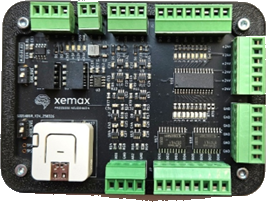
\includegraphics[width=1.0\textwidth]{graphics/xLH-io-base}
                        \end{figure}
                    \end{column}
                \end{columns}
            \end{frame}

            \begin{frame}{xLH-io-base: Features}
                \begin{columns}
                    \begin{column}{0.75\textwidth}
                        %! Author = tru
%! Date = 11.06.2025

\begin{itemize}
    \item Microcontroller M5-Stack Atom Lite
    \item 8 digitale Eingänge 24VDC
    \item 8 digitale Ausgänge 24VDC
    \item 2 analoge Eingänge 0-10VDC
    \item 2 analoge Ausgänge 0-10VDC
    \item Spannungsversorgung für xLH-lx-base integriert
    \item kompakte Umsetzung
\end{itemize}

                    \end{column}
                    \begin{column}{0.25\textwidth}
                        \begin{figure}[h]
                            \centering
                            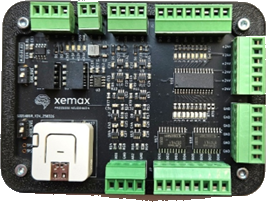
\includegraphics[width=1.0\textwidth]{graphics/xLH-io-base}
                        \end{figure}
                    \end{column}
                \end{columns}
            \end{frame}

        \subsection{xLH-io-base-sp-4}
            \begin{frame}{xLH-io-base-sp-4: Beschreibung}
                \begin{columns}
                    \begin{column}{0.75\textwidth}
                        %! Author = tru
%! Date = 11.06.2025

Der xLH-io-base-sp-4 erlaubt die Integration von bestehender Infrastruktur via Laborsteckern.

                    \end{column}
                    \begin{column}{0.25\textwidth}
                        \begin{figure}[h]
                            \centering
                            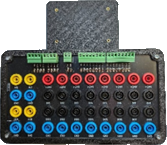
\includegraphics[width=1.0\textwidth]{graphics/xLH-io-base-sp-4}
                        \end{figure}
                    \end{column}
                \end{columns}
            \end{frame}

            \begin{frame}{xLH-io-base-sp-4: Features}
                \begin{columns}
                    \begin{column}{0.75\textwidth}
                        %! Author = tru
%! Date = 11.06.2025

\begin{itemize}
    \item 8 digitale Eingänge 24VDC
    \item 8 digitale Ausgänge 24VDC
    \item 2 analoge Eingänge 0-10VDC
    \item 2 analoge Ausgänge 0-10VDC
\end{itemize}

                    \end{column}
                    \begin{column}{0.25\textwidth}
                        \begin{figure}[h]
                            \centering
                            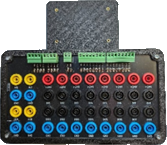
\includegraphics[width=1.0\textwidth]{graphics/xLH-io-base-sp-4}
                        \end{figure}
                    \end{column}
                \end{columns}
            \end{frame}

\end{document}
